% Options for packages loaded elsewhere
\PassOptionsToPackage{unicode}{hyperref}
\PassOptionsToPackage{hyphens}{url}
%
\documentclass[
  12pt,a4paper,lualatex,ja=standard]{bxjsarticle}
\usepackage{lmodern}
\usepackage{amsmath}
\usepackage{ifxetex,ifluatex}
\ifnum 0\ifxetex 1\fi\ifluatex 1\fi=0 % if pdftex
  \usepackage[T1]{fontenc}
  \usepackage[utf8]{inputenc}
  \usepackage{textcomp} % provide euro and other symbols
  \usepackage{amssymb}
\else % if luatex or xetex
  \usepackage{unicode-math}
  \defaultfontfeatures{Scale=MatchLowercase}
  \defaultfontfeatures[\rmfamily]{Ligatures=TeX,Scale=1}
\fi
% Use upquote if available, for straight quotes in verbatim environments
\IfFileExists{upquote.sty}{\usepackage{upquote}}{}
\IfFileExists{microtype.sty}{% use microtype if available
  \usepackage[]{microtype}
  \UseMicrotypeSet[protrusion]{basicmath} % disable protrusion for tt fonts
}{}
\makeatletter
\@ifundefined{KOMAClassName}{% if non-KOMA class
  \IfFileExists{parskip.sty}{%
    \usepackage{parskip}
  }{% else
    \setlength{\parindent}{0pt}
    \setlength{\parskip}{6pt plus 2pt minus 1pt}}
}{% if KOMA class
  \KOMAoptions{parskip=half}}
\makeatother
\usepackage{xcolor}
\IfFileExists{xurl.sty}{\usepackage{xurl}}{} % add URL line breaks if available
\IfFileExists{bookmark.sty}{\usepackage{bookmark}}{\usepackage{hyperref}}
\hypersetup{
  hidelinks,
  pdfcreator={LaTeX via pandoc}}
\urlstyle{same} % disable monospaced font for URLs
\usepackage{graphicx}
\makeatletter
\def\maxwidth{\ifdim\Gin@nat@width>\linewidth\linewidth\else\Gin@nat@width\fi}
\def\maxheight{\ifdim\Gin@nat@height>\textheight\textheight\else\Gin@nat@height\fi}
\makeatother
% Scale images if necessary, so that they will not overflow the page
% margins by default, and it is still possible to overwrite the defaults
% using explicit options in \includegraphics[width, height, ...]{}
\setkeys{Gin}{width=\maxwidth,height=\maxheight,keepaspectratio}
% Set default figure placement to htbp
\makeatletter
\def\fps@figure{htbp}
\makeatother
\setlength{\emergencystretch}{3em} % prevent overfull lines
\providecommand{\tightlist}{%
  \setlength{\itemsep}{0pt}\setlength{\parskip}{0pt}}
\setcounter{secnumdepth}{-\maxdimen} % remove section numbering
\usepackage{indentfirst}
\parindent = 1em
\usepackage{dcolumn}
\newcolumntype{.}{D{.}{.}{-1}}
\usepackage{caption}
\captionsetup[table]{name=表}
\captionsetup[figure]{name=図}
\usepackage{hyperref}
\pagestyle{empty}
\usepackage{multicol}
\usepackage{ascmac}
\setpagelayout*{top=10truemm,bottom=30truemm,left=10truemm,right=10truemm}
\usepackage{tikz}
\usetikzlibrary{arrows.meta,decorations,decorations.pathreplacing,arrows,calc}
\usepackage{tabstackengine}
\usepackage{xcolor}
\usepackage{rotating}
\usepackage{txfonts}
\usepackage{fancybox}
\usepackage{dashbox}
\usepackage{tcolorbox}
\tcbuselibrary{theorems,skins}
\usepackage{siunitx}
\usepackage{framed}
\usepackage{enumerate}
\usepackage{lastpage}
\usepackage{pgfplots}
\pgfplotsset{compat=1.15}
\usepackage{mathrsfs}
\ifluatex
  \usepackage{selnolig}  % disable illegal ligatures
\fi

\author{}
\date{\vspace{-2.5em}}

\begin{document}

\renewcommand{\thefootnote}{}
\newcounter{kaunta}
\renewcommand{\thekaunta}{\arabic{kaunta}}
\newcommand{\kaunta}{\refstepcounter{kaunta}%
\thekaunta}
\def\question{\noindent\fbox{\large\makebox[1em]{\text{\kaunta}}} \hspace{1pt}}
\newcounter{skaunta}
\renewcommand{\theskaunta}{\arabic{skaunta}}
\newcommand{\skaunta}{\refstepcounter{skaunta}%
\theskaunta}
\def\squestion{(\text{\skaunta})\hspace{2.5pt}}
\newcommand{\maru}[1]{\raise0.2ex\hbox{\textcircled{\scriptsize{#1}}}}
\newcommand{\jsim}{\mathrel{\text{∽}}}
\newcommand{\jpara}{/\!/}

\newcounter{kcounter}
\setcounter{kcounter}{0}
\newcommand{\kana}{\refstepcounter{kcounter}\ifthenelse{\value{kcounter}=1}{ア}{\ifthenelse{\value{kcounter}=2}{イ}{\ifthenelse{\value{kcounter}=3}{ウ}{\ifthenelse{\value{kcounter}=4}{エ}{\ifthenelse{\value{kcounter}=5}{オ} {\ifthenelse{\value{kcounter}=6}{カ}{\ifthenelse{\value{kcounter}=7}{キ}{\ifthenelse{\value{kcounter}=8}{ク}{\ifthenelse{\value{kcounter}=9}{ケ}{\ifthenelse{\value{kcounter}=10}{コ}{\ifthenelse{\value{kcounter}=11}{サ}{\ifthenelse{\value{kcounter}=12}{シ}{\ifthenelse{\value{kcounter}=13}{ス}{\ifthenelse{\value{kcounter}=14}{セ}{\ifthenelse{\value{kcounter}=15}{ソ}{\ifthenelse{\value{kcounter}=16}{タ}{\ifthenelse{\value{kcounter}=17}{チ}{\ifthenelse{\value{kcounter}=18}{ツ}{\ifthenelse{\value{kcounter}=19}{テ}{\ifthenelse{\value{kcounter}=20}{ト}{\ifthenelse{\value{kcounter}=21}{ナ}{\ifthenelse{\value{kcounter}=22}{ニ}{\ifthenelse{\value{kcounter}=23}{ヌ}{\ifthenelse{\value{kcounter}=24}{ネ}{\ifthenelse{\value{kcounter}=25}{ノ}{\ifthenelse{\value{kcounter}=26}{ハ}{\ifthenelse{\value{kcounter}=27}{ヒ}{\ifthenelse{\value{kcounter}=28}{フ}{\ifthenelse{\value{kcounter}=29}{ヘ}{\ifthenelse{\value{kcounter}=30}{ホ}{\ifthenelse{\value{kcounter}=31}{マ}{\ifthenelse{\value{kcounter}=32}{ミ}{\ifthenelse{\value{kcounter}=33}{ム}{\ifthenelse{\value{kcounter}=34}{メ}{\ifthenelse{\value{kcounter}=35}{モ}{\ifthenelse{\value{kcounter}=36}{ヤ}{\ifthenelse{\value{kcounter}=37}{ユ}{\ifthenelse{\value{kcounter}=38}{ヨ}{\ifthenelse{\value{kcounter}=39}{ラ}{\ifthenelse{\value{kcounter}=40}{リ}{\ifthenelse{\value{kcounter}=41}{ル}{\ifthenelse{\value{kcounter}=42}{レ}{\ifthenelse{\value{kcounter}=43}{ロ}{\ifthenelse{\value{kcounter}=44}{ワ}{・}}}}}}}}}}}}}}}}}}}}}}}}}}}}}}}}}}}}}}}}}}}}}

\newcommand{\kuran}[1]{\framebox[1.5cm][c]{\maru{\kana}}}

\newcommand{\degre}{\ensuremath{^\circ}}

\newcommand{\myarc}[1]{
   \tikz [baseline = (N.base), every node/.style={}] {
      \node [inner sep = 0pt] (N) {$\mathrm{#1}$};
      \draw [line width = 0.4pt] plot [smooth, tension=1.3] coordinates {
         ($(N.north west) + (0.1ex,0)$)
         ($(N.north)      + (0,0.5ex)$)
         ($(N.north east) + (0,0)$)
      };
   }
}

\makeatletter
\newenvironment{figurehere}{\def\@captype{figure}}{}
\makeatother

\newcommand{\goku}[1]{\, \fbox{\phantom{\text{#1}} \quad} \,}

\hypertarget{ux7acbux4f53ux306eux898bux65b9ux3068ux8abfux3079ux65b9raise-0.2exhboxtextcircledscriptsize2}{%
\subsection{\texorpdfstring{立体の見方と調べ方\(\raise 0.2ex\hbox{\textcircled{\scriptsize{2}}}\)}{立体の見方と調べ方\textbackslash raise 0.2ex\textbackslash hbox\{\textbackslash textcircled\{\textbackslash scriptsize\{2\}\}\}}}\label{ux7acbux4f53ux306eux898bux65b9ux3068ux8abfux3079ux65b9raise-0.2exhboxtextcircledscriptsize2}}

\begin{multicols}{2}
右の図の直方体で、線分AGをこの直方体の\, \fbox{\phantom{\text{対角線}} \quad} \,という。BH, CE, DFも対角線である。

\columnbreak

\begin{center}
\def\@captype{figure}
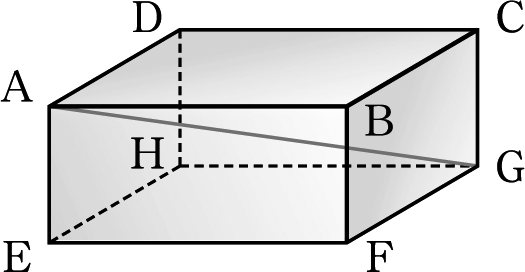
\includegraphics{media/image35.png}

\end{center}
\end{multicols}

\begin{multicols}{2}

平面Pに対して、どの方向にも傾いていない直線$l$を考えよう。このとき、$l$はPとの交点Oを通る上のどの直線にも\, \fbox{\phantom{\text{垂直}} \quad} \,になっている。このようなとき、直線$l$は平面Pに\, \fbox{\phantom{\text{垂直である}} \quad} \,という。

\columnbreak

\begin{center}

\includegraphics{media/image46.png}
\end{center}
\end{multicols}

\begin{multicols}{2}

平面Pと交わる直線$l$がその交点Oを通るP上の異なる2つの直線$m, \, n$に垂直になっていれば、直線$l$は平面Pに\, \fbox{\phantom{\text{垂直である}} \quad} \,。

\columnbreak

\begin{center}
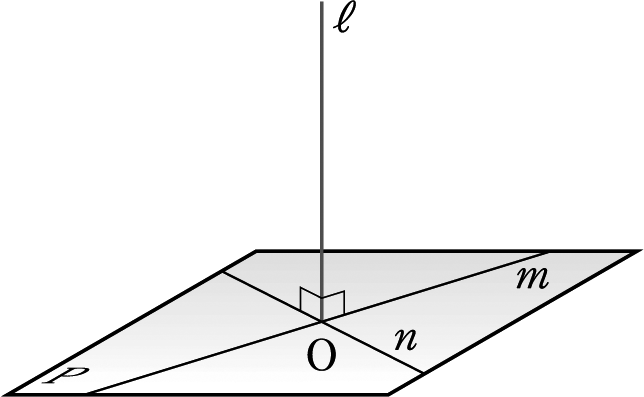
\includegraphics{media/image49.png}
\end{center}
\end{multicols}

\begin{multicols}{2}
2つの平面P, Qが交わるとき、交線$l$上の点で、それぞれの平面上にひいた2つの垂線のつくる角を平面P, Qのつくる\, \fbox{\phantom{\text{角}} \quad} \,という。

\columnbreak

\begin{center}
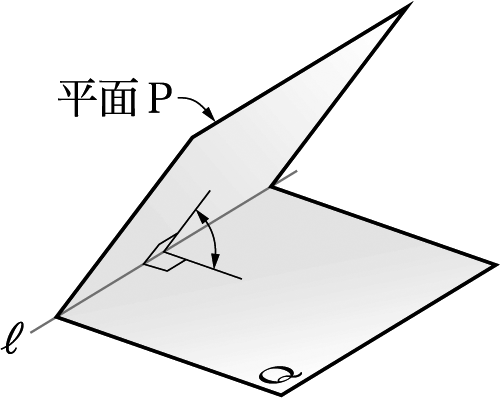
\includegraphics{media/image60.png}
\end{center}

\end{multicols}

\begin{multicols}{2}
2つの平面P, Qのつくる角が直角のとき、その2つの平面P, Qは垂直であるといい、\, \fbox{\phantom{\text{P$\perp$Q}} \quad} \,と表す。

平面Pに垂直な直線をふくむ平面は、平面Pに\, \fbox{\phantom{\text{垂直である}} \quad} \,。

\columnbreak

\begin{center}
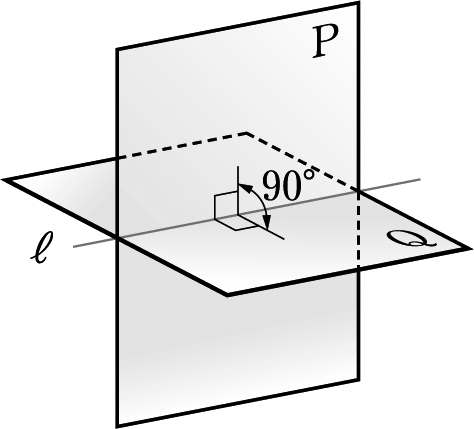
\includegraphics{media/image63.png}
\end{center}
\end{multicols}

\newpage

\begin{multicols}{2}
右の図は長方形の紙を二つ折にして机の面Pに立てた図に、記号をつけたものです。折り目の直線EFは平面Pに垂直である。なぜなら、四角形ABFE, DCFEは長方形であるから、\, \fbox{\phantom{\text{EF$\perp$BF}} \quad} \,, EF$\perp$CFとなる。平面Pと交わる直線EFがその交点Fを通るP上の異なる2つの直線BF, CFに垂直になっているから、直線EFは平面Pに\, \fbox{\phantom{\text{垂直である}} \quad} \,。

また、平面ABEF, EFCDは平面Pに垂直な直線EFをふくむから、平面Pに\, \fbox{\phantom{\text{垂直である}} \quad} \,。

\columnbreak

\begin{center}

\includegraphics{media/image57.png}
\end{center}
\end{multicols}

\begin{multicols}{2}
1つの点Aから平面Pにひいた垂線と、Pとの交点をHとするとき、線分AHの\, \fbox{\phantom{\text{長さ}} \quad} \,を、点Aと\, \fbox{\phantom{\text{平面Pとの距離}} \quad} \,という。

\columnbreak

\begin{center}
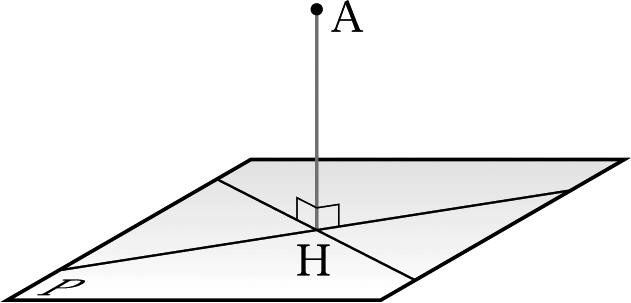
\includegraphics{media/image78.png}
\end{center}

\end{multicols}

\vspace{10mm}

\begin{multicols}{2}
平行な平面について、一方の平面上の点ともう一方の平面との距離は\, \fbox{\phantom{\text{すべて等しい}} \quad} \,。この距離を\, \fbox{\phantom{\text{平面と平面の距離}} \quad} \,という。

\columnbreak

\begin{center}
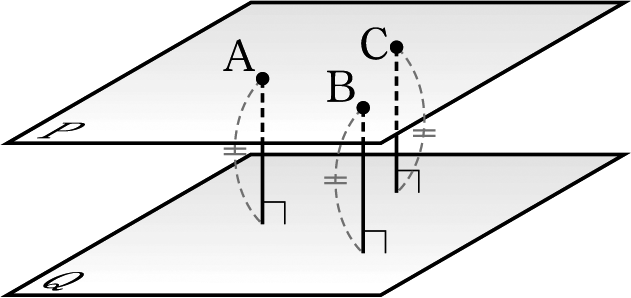
\includegraphics{media/image80.png}
\end{center}
\end{multicols}

角柱や円柱では、2つの底面は平行で、一方の底面ともう一方の底面との距離が、その角柱や円柱の\, \fbox{\phantom{\text{高さ}} \quad} \,である。角錐や円錐では、底面とそれに対する\, \fbox{\phantom{\text{頂点との距離}} \quad} \,がその高さである。

\begin{center}
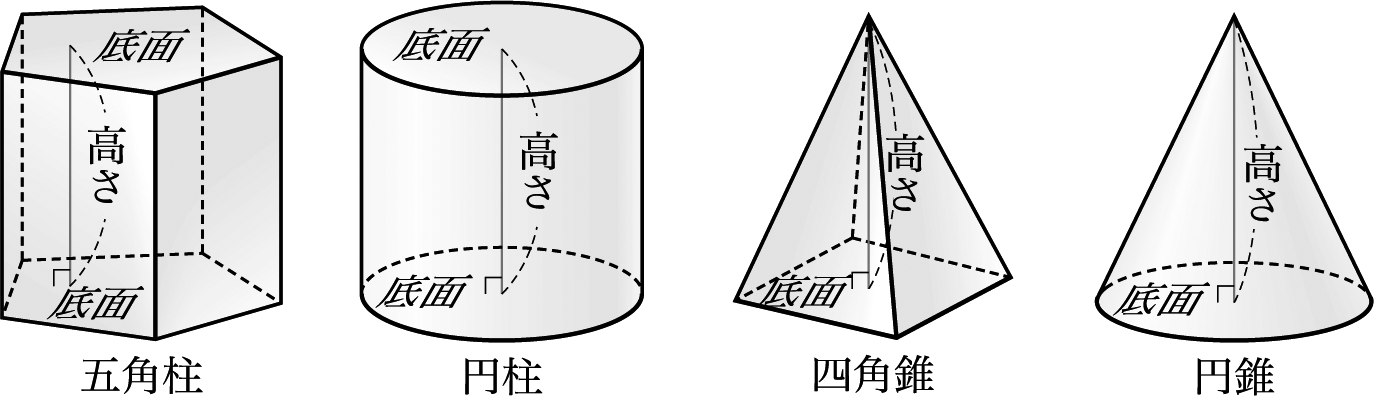
\includegraphics{media/image82.png}
\end{center}

\newpage

下の図のように、点が動くことによって、\, \fbox{\phantom{\text{線}} \quad} \,ができる。また、線が動くことによって\, \fbox{\phantom{\text{面}} \quad} \,ができる。さらに、面が動くことによって\, \fbox{\phantom{\text{立体}} \quad} \,ができる。

\begin{center}
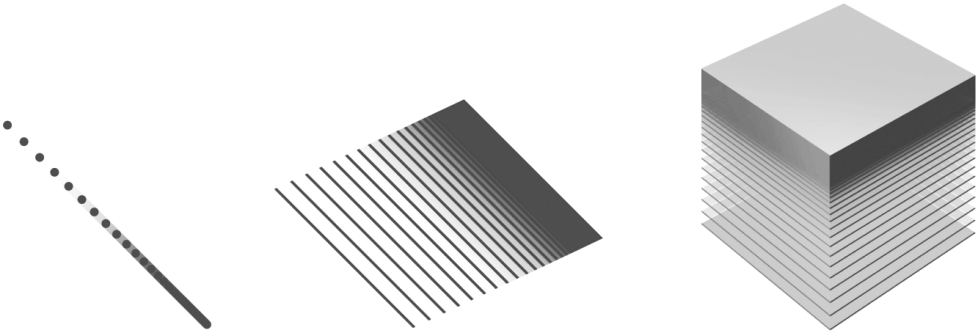
\includegraphics{media/image87.png}
\end{center}

角柱や円柱は、底面がそれと垂直な方向に動いてできた立体とも考えられる。底面の周の動いたあとは、その立体の\, \fbox{\phantom{\text{側面}} \quad} \,であり、動いた距離が\, \fbox{\phantom{\text{高さ}} \quad} \,である。

\begin{center}
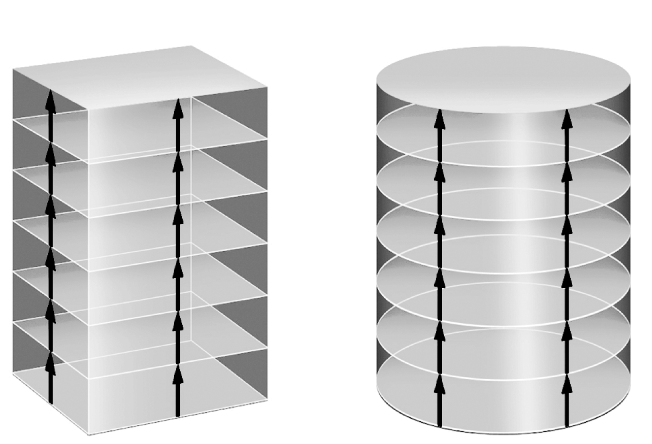
\includegraphics{media/image88.png}
\hspace{8mm}
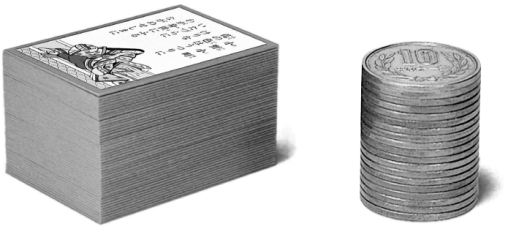
\includegraphics{media/image89.png}
\end{center}

円柱や円錐は、それぞれ長方形や直角三角形を空間で\, \fbox{\phantom{\text{回転させて}} \quad} \,できた立体と考えることができる。このとき、円柱や円錐の側面をえがく線分ABを円柱や円錐の\, \fbox{\phantom{\text{母線}} \quad} \,という。

\begin{center}
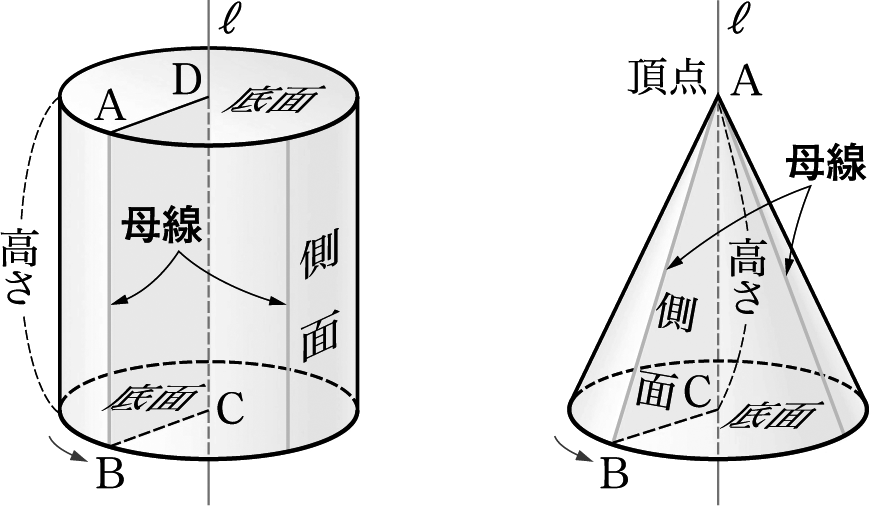
\includegraphics{media/image102.png}
\end{center}

\begin{multicols}{2}
円柱や円錐のように、1つの直線を軸として平面図形を回転させてできる立体を\, \fbox{\phantom{\text{回転体}} \quad} \,という。球は、\, \fbox{\phantom{\text{半円}} \quad} \,をその\, \fbox{\phantom{\text{直径}} \quad} \,を軸として回転させてできた回転体である。

\columnbreak

\begin{center}
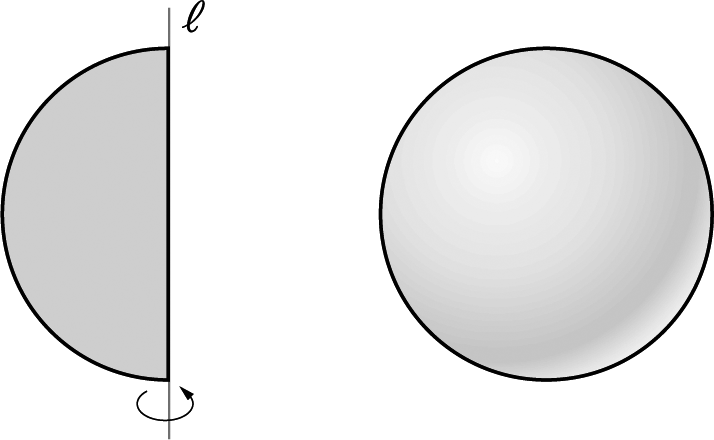
\includegraphics{media/image104.png}
\end{center}
\end{multicols}

\begin{multicols}{2}
回転体を\, \fbox{\phantom{\text{回転の軸をふくむ}} \quad} \,平面で切ると、その切り口は、回転の軸を\, \fbox{\phantom{\text{対称の軸}} \quad} \,とする\, \fbox{\phantom{\text{線対称}} \quad} \,な図形となる。

\columnbreak

\begin{center}

\includegraphics{media/image105.png}
\end{center}
\end{multicols}

\end{document}
